\documentclass[11pt,a4paper]{article}

% --- Packages ---
\usepackage[utf8]{inputenc}
\usepackage[T1]{fontenc}
\usepackage{lmodern}
\usepackage{amsmath,amssymb,amsfonts}
\usepackage{booktabs}
\usepackage{xcolor}
\usepackage{geometry}
\usepackage{titlesec}
\usepackage{hyperref}
\usepackage{microtype}
\usepackage{graphicx}
\usepackage{caption}
\usepackage{subcaption}
\usepackage{multirow}
\usepackage{enumitem}

\geometry{margin=1in}

% --- Custom Colors ---
\definecolor{primaryblue}{HTML}{1A365D}
\definecolor{secondarygreen}{HTML}{2F855A}
\definecolor{alertred}{HTML}{9B2C2C}
\definecolor{notegray}{HTML}{4A5568}

\hypersetup{
    colorlinks=true,
    linkcolor=primaryblue,
    urlcolor=primaryblue,
    citecolor=secondarygreen
}

% --- Section Styling ---
\titleformat{\section}{\large\bfseries\color{primaryblue}}{\thesection}{1em}{}
\titleformat{\subsection}{\normalsize\bfseries\color{secondarygreen}}{\thesubsection}{1em}{}

% --- Theorem Environments ---
\newtheorem{proposition}{Proposition}
\newtheorem{proof}{Proof}

\title{\textbf{Activation Geometry, Plasticity, and Out-of-Distribution Generalization}\\ \large Master Report: Radial Suppression Experiments \\ \normalsize Last Updated: July 29, 2026}
\author{}
\date{}

\begin{document}

\maketitle

\begin{abstract}
This is the master tracking document for all theoretical and empirical work on the activation norm penalty ($L_{\text{norm}}$) / Radial Suppression (RS) framework. It compiles theoretical proofs, detailed experimental results from Srijan (local experiments on plasticity and distribution shift), Harshit (spurious correlations and OOD robustness on CelebA, Camelyon17, and Spawrious), Sarthak (continual learning on Split CIFAR-100 with architectural ablations), and Aaditya (fine-tuning pretrained ViTs on VTAB-1k splits). The document concludes with a synthesis of what the results tell us, what they don't, and detailed next steps for continuing the research.
\end{abstract}

\newpage
\tableofcontents
\newpage

% ==============================================================================
\section{Theoretical Foundations}
\label{sec:theory}
% ==============================================================================

The fundamental objective of the activation norm penalty is to restrict the radial expansion of hidden activations, forcing gradient descent to optimize along angular (tangential) directions. Given a neural network layer with pre-activations $h \in \mathbb{R}^d$, the augmented loss objective is formulated as:
\begin{equation}
\label{eq:total_loss}
L_{\text{total}} = L_{\text{CE}}(f(x;\theta), y) + \lambda\, L_{\text{norm}}(h)
\end{equation}
where:
\begin{equation}
\label{eq:norm_penalty}
L_{\text{norm}}(h) = \frac{1}{d}\left(\|h\|_2 - \sqrt{d}\right)^2
\end{equation}
The target scaling factor $\sqrt{d}$ aligns the constraint with standard $\mathcal{O}(1)$ initialization variance, ensuring that width scaling does not trigger activation explosion or collapse.

Below, we detail the formal derivations of the three propositions establishing the connection between activation norms, parameter sharpness, optimization manifold projection, and spectral dimensionality.

% ------------------------------------------------------------------------------
\subsection{Proposition 1: Preempting the Edge of Stability via Radial Bounding}
\textbf{Proposition 1.} \textit{Radial inflation in activation space drives progressive sharpening in parameter space. Constraining activation norms bounds the parameter spectral norm, formally preempting the Edge of Stability (EoS) instability threshold.}

\paragraph{Proof.} Let a single-layer linear approximation of the network activations be $h = Wx$, where $W \in \mathbb{R}^{d \times d_{\text{in}}}$ is the weight matrix and $x$ is the input from the preceding layer. The cross-entropy loss $L_{\text{CE}}$ operates on the logits, which are downstream linear mappings of $h$. Let $\ell(h)$ represent the mapping from pre-activations to the scalar loss.

Applying the chain rule, the gradient of the loss with respect to the weights is:
\begin{equation}
\nabla_W L_{\text{CE}} = (\nabla_h \ell) x^T
\end{equation}
The Hessian matrix with respect to the weights $H_W$, omitting the second-derivative tensor terms of the network (which are negligible near convergence under local linearity), is given by the Kronecker product of the pre-activation Hessian and the input outer product:
\begin{equation}
H_W \approx (\nabla^2_h \ell) \otimes (x x^T)
\end{equation}
Under standard cross-entropy, the magnitude of the activations grows without bound ($\|h\|_2 \to \infty$) to push the logits into the saturating regime of the softmax function. Since $h = Wx$, this radial inflation requires the weights to grow in norm:
\begin{equation}
\|W\|_F \to \infty
\end{equation}
As weight magnitude scales up, the maximal eigenvalue of the parameter Hessian $\lambda_{\text{max}}(H_W)$ increases proportionally. The Edge of Stability (EoS) framework states that gradient descent enters an unstable, self-correcting regime when $\lambda_{\text{max}}(H_W) > 2/\eta$, where $\eta$ is the learning rate.

By introducing the activation norm penalty, the constraint enforces:
\begin{equation}
\|h\|_2 \approx \sqrt{d}
\end{equation}
This directly bounds the spectral norm of $W$. Because the maximal eigenvalue $\lambda_{\text{max}}(H_W)$ is bounded by functions of the bounded weight and input norms, the local sharpness is prevented from crossing the EoS threshold. This formally accounts for the massive reduction in Hessian trace observed in norm-penalized models. $\blacksquare$

% ------------------------------------------------------------------------------
\subsection{Proposition 2: Lagrangian Relaxation of Riemannian Flow}
\textbf{Proposition 2.} \textit{The activation norm penalty acts as a continuous Lagrangian relaxation of a Riemannian gradient flow on the hypersphere $\mathbb{S}^{d-1}(\sqrt{d})$, where the penalty multiplier $\lambda$ dictates the stiffness of the manifold retraction.}

\paragraph{Proof.} Consider the continuous-time gradient flow of the activation vector:
\begin{equation}
\dot{h} = -\nabla_h L_{\text{total}}
\end{equation}
Expanding the gradient of the augmented loss using Equation \ref{eq:total_loss} and \ref{eq:norm_penalty}:
\begin{equation}
\nabla_h L_{\text{total}} = \nabla_h L_{\text{CE}} + \frac{2\lambda}{d} \left( \frac{\|h\|_2 - \sqrt{d}}{\|h\|_2} \right) h
\end{equation}
Let $P_r = \frac{h h^T}{\|h\|_2^2}$ be the orthogonal projection matrix onto the radial direction of $h$. We decompose the continuous flow $\dot{h}$ into its radial ($\dot{h}_{\text{rad}}$) and tangential ($\dot{h}_{\text{tan}}$) components:
\begin{equation}
\dot{h}_{\text{rad}} = -P_r \nabla_h L_{\text{total}} = -P_r \nabla_h L_{\text{CE}} - \frac{2\lambda}{d} (\|h\|_2 - \sqrt{d}) \frac{h}{\|h\|_2}
\end{equation}
\begin{equation}
\dot{h}_{\text{tan}} = -(I - P_r) \nabla_h L_{\text{total}} = -(I - P_r) \nabla_h L_{\text{CE}}
\end{equation}
In the asymptotic limit where the penalty multiplier approaches infinity ($\lambda \to \infty$), the radial restoring force becomes infinitely stiff. Any infinitesimal radial deviation from the target radius $\sqrt{d}$ is corrected instantly:
\begin{equation}
\dot{h}_{\text{rad}} \to 0 \quad \implies \quad \|h\|_2 \to \sqrt{d}
\end{equation}
In this limit, the overall dynamics of $h$ reduce exactly to the projection:
\begin{equation}
\dot{h} = -(I - P_r) \nabla_h L_{\text{CE}}
\end{equation}
This is the formal definition of a Riemannian gradient flow restricted to the hypersphere $\mathbb{S}^{d-1}(\sqrt{d})$. For finite values of $\lambda$, the soft norm penalty operates as a continuous Lagrangian relaxation, avoiding the computational complexity and optimization bottlenecks of hard projection retractions while preserving the favorable tangential gradient dynamics. $\blacksquare$

% ------------------------------------------------------------------------------
\subsection{Proposition 3: Spectral Collapse and Antagonistic Gradients}
\textbf{Proposition 3.} \textit{Unconstrained cross-entropy exhibits an implicit bias toward rank-1 representations. The activation penalty induces an ``antagonistic gradient'' that counteracts this bias, preserving the stable rank and allowing the spectral edge of generalizing circuits to assemble.}

\paragraph{Proof.} Let $A \in \mathbb{R}^{B \times d}$ be the activation matrix for a batch of size $B$. The representational diversity is captured by the stable rank:
\begin{equation}
s(A) = \frac{\|A\|_F^2}{\|A\|_2^2} = \frac{\sum_{i=1}^r \sigma_i^2}{\sigma_1^2}
\end{equation}
where $\sigma_i$ are the singular values of $A$. Cross-entropy optimization on separable data implicitly drives the network toward max-margin solutions, which causes the dominant singular value $\sigma_1$ to inflate exponentially faster than the trailing singular values ($\sigma_2, \dots, \sigma_r$), collapsing the stable rank $s(A) \to 1$.

The gradient of the norm penalty with respect to the hidden activations is:
\begin{equation}
\nabla_h L_{\text{norm}} = \frac{2}{d}(\|h\|_2 - \sqrt{d})\frac{h}{\|h\|_2}
\end{equation}
Because this gradient vector is collinear with $h$, its projection is maximal along the directions corresponding to the dominant activations in the batch. Under Singular Value Decomposition (SVD), the dominant singular value $\sigma_1$ corresponds to the direction of maximum variance of the activations.

The penalty gradient acts as a restoring force directly opposing this inflation direction, exerting its largest suppressive force along the principal eigenvector of $A^T A$. This constant radial pullback limits the growth of $\sigma_1$, distributing the gradient updates across the orthogonal subspaces of the trailing singular values ($\sigma_2, \dots, \sigma_r$). This antagonistic gradient preserves the stable rank $s(A) \gg 1$, keeping the latent representation space high-dimensional and permitting the formation of multi-frequency generalizing circuits. $\blacksquare$

\newpage

% ==============================================================================
\section{Local Experiments (Srijan): Plasticity and Shifting Distributions}
\label{sec:local}
% ==============================================================================

Our local experiments evaluated $L_{\text{norm}}$ in sequential learning settings where representation saturation acts as the bottleneck. All experiments were conducted using PyTorch on a single NVIDIA RTX A6000 GPU.

% ------------------------------------------------------------------------------
\subsection{Experiment 1: Permuted MNIST v2 (MLP Scale Test)}
\textbf{Setup:} We trained a narrow 3-layer MLP ($d_{\text{hidden}} = 128$) sequentially on $20$ tasks (each task is a unique pixel permutation of MNIST) for $10$ epochs per task ($200$ epochs total) using AdamW ($lr=10^{-3}$, $WD=10^{-3}$, batch size $256$). The narrow width and increased depth were chosen to create capacity bottlenecks and promote saturation.

\textbf{Baselines Compared:}
\begin{enumerate}
    \item \textbf{Baseline:} Standard Cross-Entropy with weak Weight Decay ($10^{-3}$).
    \item \textbf{Strong WD:} Standard Cross-Entropy with strong Weight Decay ($10^{-1}$).
    \item \textbf{L2-Init:} Regularizing weights toward initial parameters ($\alpha=0.01$).
    \item \textbf{Shrink \& Perturb (S\&P):} Shrinking weights by $0.8$ and adding noise ($\sigma=0.01$) at task boundaries.
    \item \textbf{Norm Penalty:} Activation norm penalty ($\lambda=0.05$) applied to all hidden layers.
    \item \textbf{Continual Backpropagation (CB):} Resets utilities of neurons below a threshold ($\tau=0.01$, $\eta=0.01$) based on Dohare et al. (2024).
    \item \textbf{Norm Penalty + CB:} The combination of prevention ($L_{\text{norm}}$) and reset (CB).
\end{enumerate}

\textbf{Results:} As shown in Table \ref{tab:permuted_mnist_v2}, standard training suffers from severe capacity decay, resulting in $40.97\%$ dead neurons across the network by Task 20. The norm penalty completely eliminates neuron death ($0.00\%$), maintaining a high representation rank ($71.81$ vs. $32.97$). S\&P yields the highest final accuracy ($97.84\%$), but does not fully solve the dead neuron issue ($15.36\%$). The combination of Norm Penalty + CB successfully keeps dead neurons at exactly $0.00\%$.

\begin{table}[ht]
\centering
\caption{Permuted MNIST v2 results (3-layer MLP, 20 tasks, 3 seeds).}
\label{tab:permuted_mnist_v2}
\resizebox{\columnwidth}{!}{%
\begin{tabular}{lcccc}
\toprule
\textbf{Method} & \textbf{Task 20 Acc (\%)} & \textbf{Task 1 Acc (\%)} & \textbf{Dead Neurons \%} & \textbf{Eff. Rank} \\
\midrule
Baseline & $96.83 \pm 0.16$ & $8.88 \pm 1.12$ & $40.97 \pm 5.66$ & $32.97 \pm 2.42$ \\
Strong WD ($10^{-1}$) & $97.55 \pm 0.02$ & $10.82 \pm 1.10$ & $25.17 \pm 0.86$ & $28.97 \pm 0.67$ \\
L2-Init & $94.17 \pm 0.24$ & $10.27 \pm 1.02$ & $1.82 \pm 0.97$ & $25.05 \pm 0.48$ \\
Shrink \& Perturb & $\mathbf{97.84 \pm 0.08}$ & $10.02 \pm 1.07$ & $15.36 \pm 0.97$ & $34.77 \pm 0.49$ \\
Norm Penalty & $97.18 \pm 0.19$ & $6.85 \pm 0.99$ & $\mathbf{0.00 \pm 0.00}$ & $\mathbf{71.81 \pm 0.09}$ \\
Continual Backprop & $97.58 \pm 0.08$ & $\mathbf{10.15 \pm 1.50}$ & $17.45 \pm 1.53$ & $38.00 \pm 0.39$ \\
Norm Penalty + CB & $97.24 \pm 0.16$ & $9.46 \pm 1.63$ & $\mathbf{0.00 \pm 0.00}$ & $71.27 \pm 0.07$ \\
\bottomrule
\end{tabular}%
}
\end{table}

% ------------------------------------------------------------------------------
\subsection{Experiment 2: Split CIFAR-10 (CNN Backbone)}
\textbf{Setup:} We split CIFAR-10 into $5$ sequential tasks of $2$ classes each. We trained a 4-layer CNN (no BatchNorm) with task-specific classification heads. The network was trained using AdamW ($lr=3\times 10^{-4}$, batch size $128$) for $40$ epochs per task.

\textbf{Results:} Norm penalty applied to all layers successfully suppressed neuron saturation, reducing dead neurons in the penultimate FC layer from $26.43\%$ to $2.86\%$, while increasing representation rank to $87.06$ (Table \ref{tab:split_cifar10}). When combining Norm Penalty + CB, we achieved exactly $0.00\%$ dead neurons. The norm penalty increases forgetting slightly (Task 1 accuracy drops to $\sim57\%$ vs. $73.68\%$ in the baseline), as keeping the representation active on the sphere makes features adapt more aggressively to new tasks, overwriting older ones.

\begin{table}[ht]
\centering
\caption{Split CIFAR-10 results (4-layer CNN, 5 tasks, 3 seeds).}
\label{tab:split_cifar10}
\resizebox{\columnwidth}{!}{%
\begin{tabular}{lcccc}
\toprule
\textbf{Method} & \textbf{Task 5 Acc (\%)} & \textbf{Task 1 Acc (\%)} & \textbf{Dead Neurons \% (FC)} & \textbf{Penult. Rank} \\
\midrule
Baseline & $95.28 \pm 0.20$ & $\mathbf{73.68 \pm 5.35}$ & $26.43 \pm 3.10$ & $56.37 \pm 2.74$ \\
Strong WD ($10^{-1}$) & $95.75 \pm 0.45$ & $69.07 \pm 9.34$ & $34.51 \pm 3.01$ & $38.41 \pm 5.64$ \\
Shrink \& Perturb & $\mathbf{96.00 \pm 0.32}$ & $67.02 \pm 7.05$ & $35.16 \pm 3.98$ & $40.08 \pm 2.33$ \\
Norm Penalty (FC only) & $95.78 \pm 0.19$ & $57.38 \pm 5.76$ & $5.60 \pm 0.18$ & $85.32 \pm 1.48$ \\
Norm Penalty (All Layers)& $95.53 \pm 0.22$ & $56.70 \pm 3.25$ & $2.86 \pm 0.74$ & $\mathbf{87.06 \pm 1.29}$ \\
Continual Backprop & $95.37 \pm 0.46$ & $72.25 \pm 4.35$ & $3.39 \pm 0.74$ & $59.33 \pm 2.04$ \\
Norm Penalty + CB & $95.73 \pm 0.25$ & $63.40 \pm 2.63$ & $\mathbf{0.00 \pm 0.00}$ & $85.94 \pm 4.83$ \\
\bottomrule
\end{tabular}%
}
\end{table}

% ------------------------------------------------------------------------------
\subsection{Experiment 3: $\tilde{\Phi}_{\text{rad}}$ as a Predictive Diagnostic}
\textbf{Setup:} We computed the Normalized Fractional Radial Energy ($\tilde{\Phi}_{\text{rad}}$) at the end of each task $t$ and correlated it post-hoc with the peak accuracy achieved on task $t+1$ using the Permuted MNIST v2 diagnostics.

\textbf{Results:} We observed a strong Pearson correlation of $r = 0.682$ ($p = 9.0 \times 10^{-5}$) under the baseline condition. This provides empirical validation that radial energy is a reliable, label-free diagnostic indicator of sequential representation decay. Under the norm penalty, this correlation is weakened ($r = 0.488$), confirming that the penalty suppresses the radial inflation dynamics.

% ------------------------------------------------------------------------------
\subsection{Experiment 4: Rotating MNIST (Continuous Domain Shift)}
\textbf{Setup:} We trained a 2-layer MLP ($d_{\text{hidden}}=256$) on MNIST digits that were continuously rotated from $0^\circ$ to $180^\circ$ over 100 epochs. Performance was evaluated on the final $178.2^\circ$ rotation test set.

\textbf{Results:} In this online domain shift setting, the norm penalty completely prevents neuron saturation, resulting in $0.00\%$ dead neurons and keeping the penultimate rank high ($122.33$ vs. $76.54$ for baseline), as reported in Table \ref{tab:rotating_mnist}.

\begin{table}[ht]
\centering
\caption{Rotating MNIST results (2-layer MLP, 100 epochs, 3 seeds).}
\label{tab:rotating_mnist}
\resizebox{\columnwidth}{!}{%
\begin{tabular}{lccc}
\toprule
\textbf{Method} & \textbf{Final Test Acc ($178.2^\circ$) (\%)} & \textbf{Dead Neurons \% ($h_2$)} & \textbf{Eff. Rank ($h_2$)} \\
\midrule
Baseline & $97.92 \pm 0.07$ & $3.39 \pm 0.80$ & $76.54 \pm 0.83$ \\
Strong WD & $\mathbf{98.29 \pm 0.14}$ & $5.08 \pm 1.15$ & $68.10 \pm 0.14$ \\
Norm Penalty & $97.98 \pm 0.16$ & $\mathbf{0.00 \pm 0.00}$ & $\mathbf{122.33 \pm 0.12}$ \\
Continual Backprop & $97.93 \pm 0.10$ & $0.26 \pm 0.18$ & $74.39 \pm 0.81$ \\
Norm Penalty + CB & $98.04 \pm 0.20$ & $\mathbf{0.00 \pm 0.00}$ & $121.62 \pm 0.30$ \\
\bottomrule
\end{tabular}%
}
\end{table}

\newpage

% ==============================================================================
\section{Harshit: Spurious Correlations and OOD Robustness}
\label{sec:harshit}
% ==============================================================================

Harshit evaluated Radial Suppression on four vision datasets characterized by strong spurious correlations. The central hypothesis, derived from Proposition 2, is that the norm penalty acts as a variance-dependent suppressor: since spurious features (like background textures) tend to be the highest-variance directions in the input, they receive the strongest regularization, allowing the model to rely on core structural features instead.

% ------------------------------------------------------------------------------
\subsection{WILDS Waterbirds (Small Data Limitation)}

The WILDS Waterbirds dataset is small ($\sim4,700$ images). Training ResNet-18 from scratch produced low performance across all conditions (Figure~\ref{fig:waterbirds}). When using a pretrained ResNet-50, an inverse effect was observed: $\lambda = 1$ actively pushed the rank down rather than preserving it.

\textbf{Takeaway:} The method requires sufficient data for the anisotropic regularization to meaningfully separate signal from noise. On tiny datasets, the penalty has nothing structurally useful to ``push'' the model toward.

\begin{figure}[ht]
\centering
\begin{subfigure}[b]{0.48\textwidth}
    \centering
    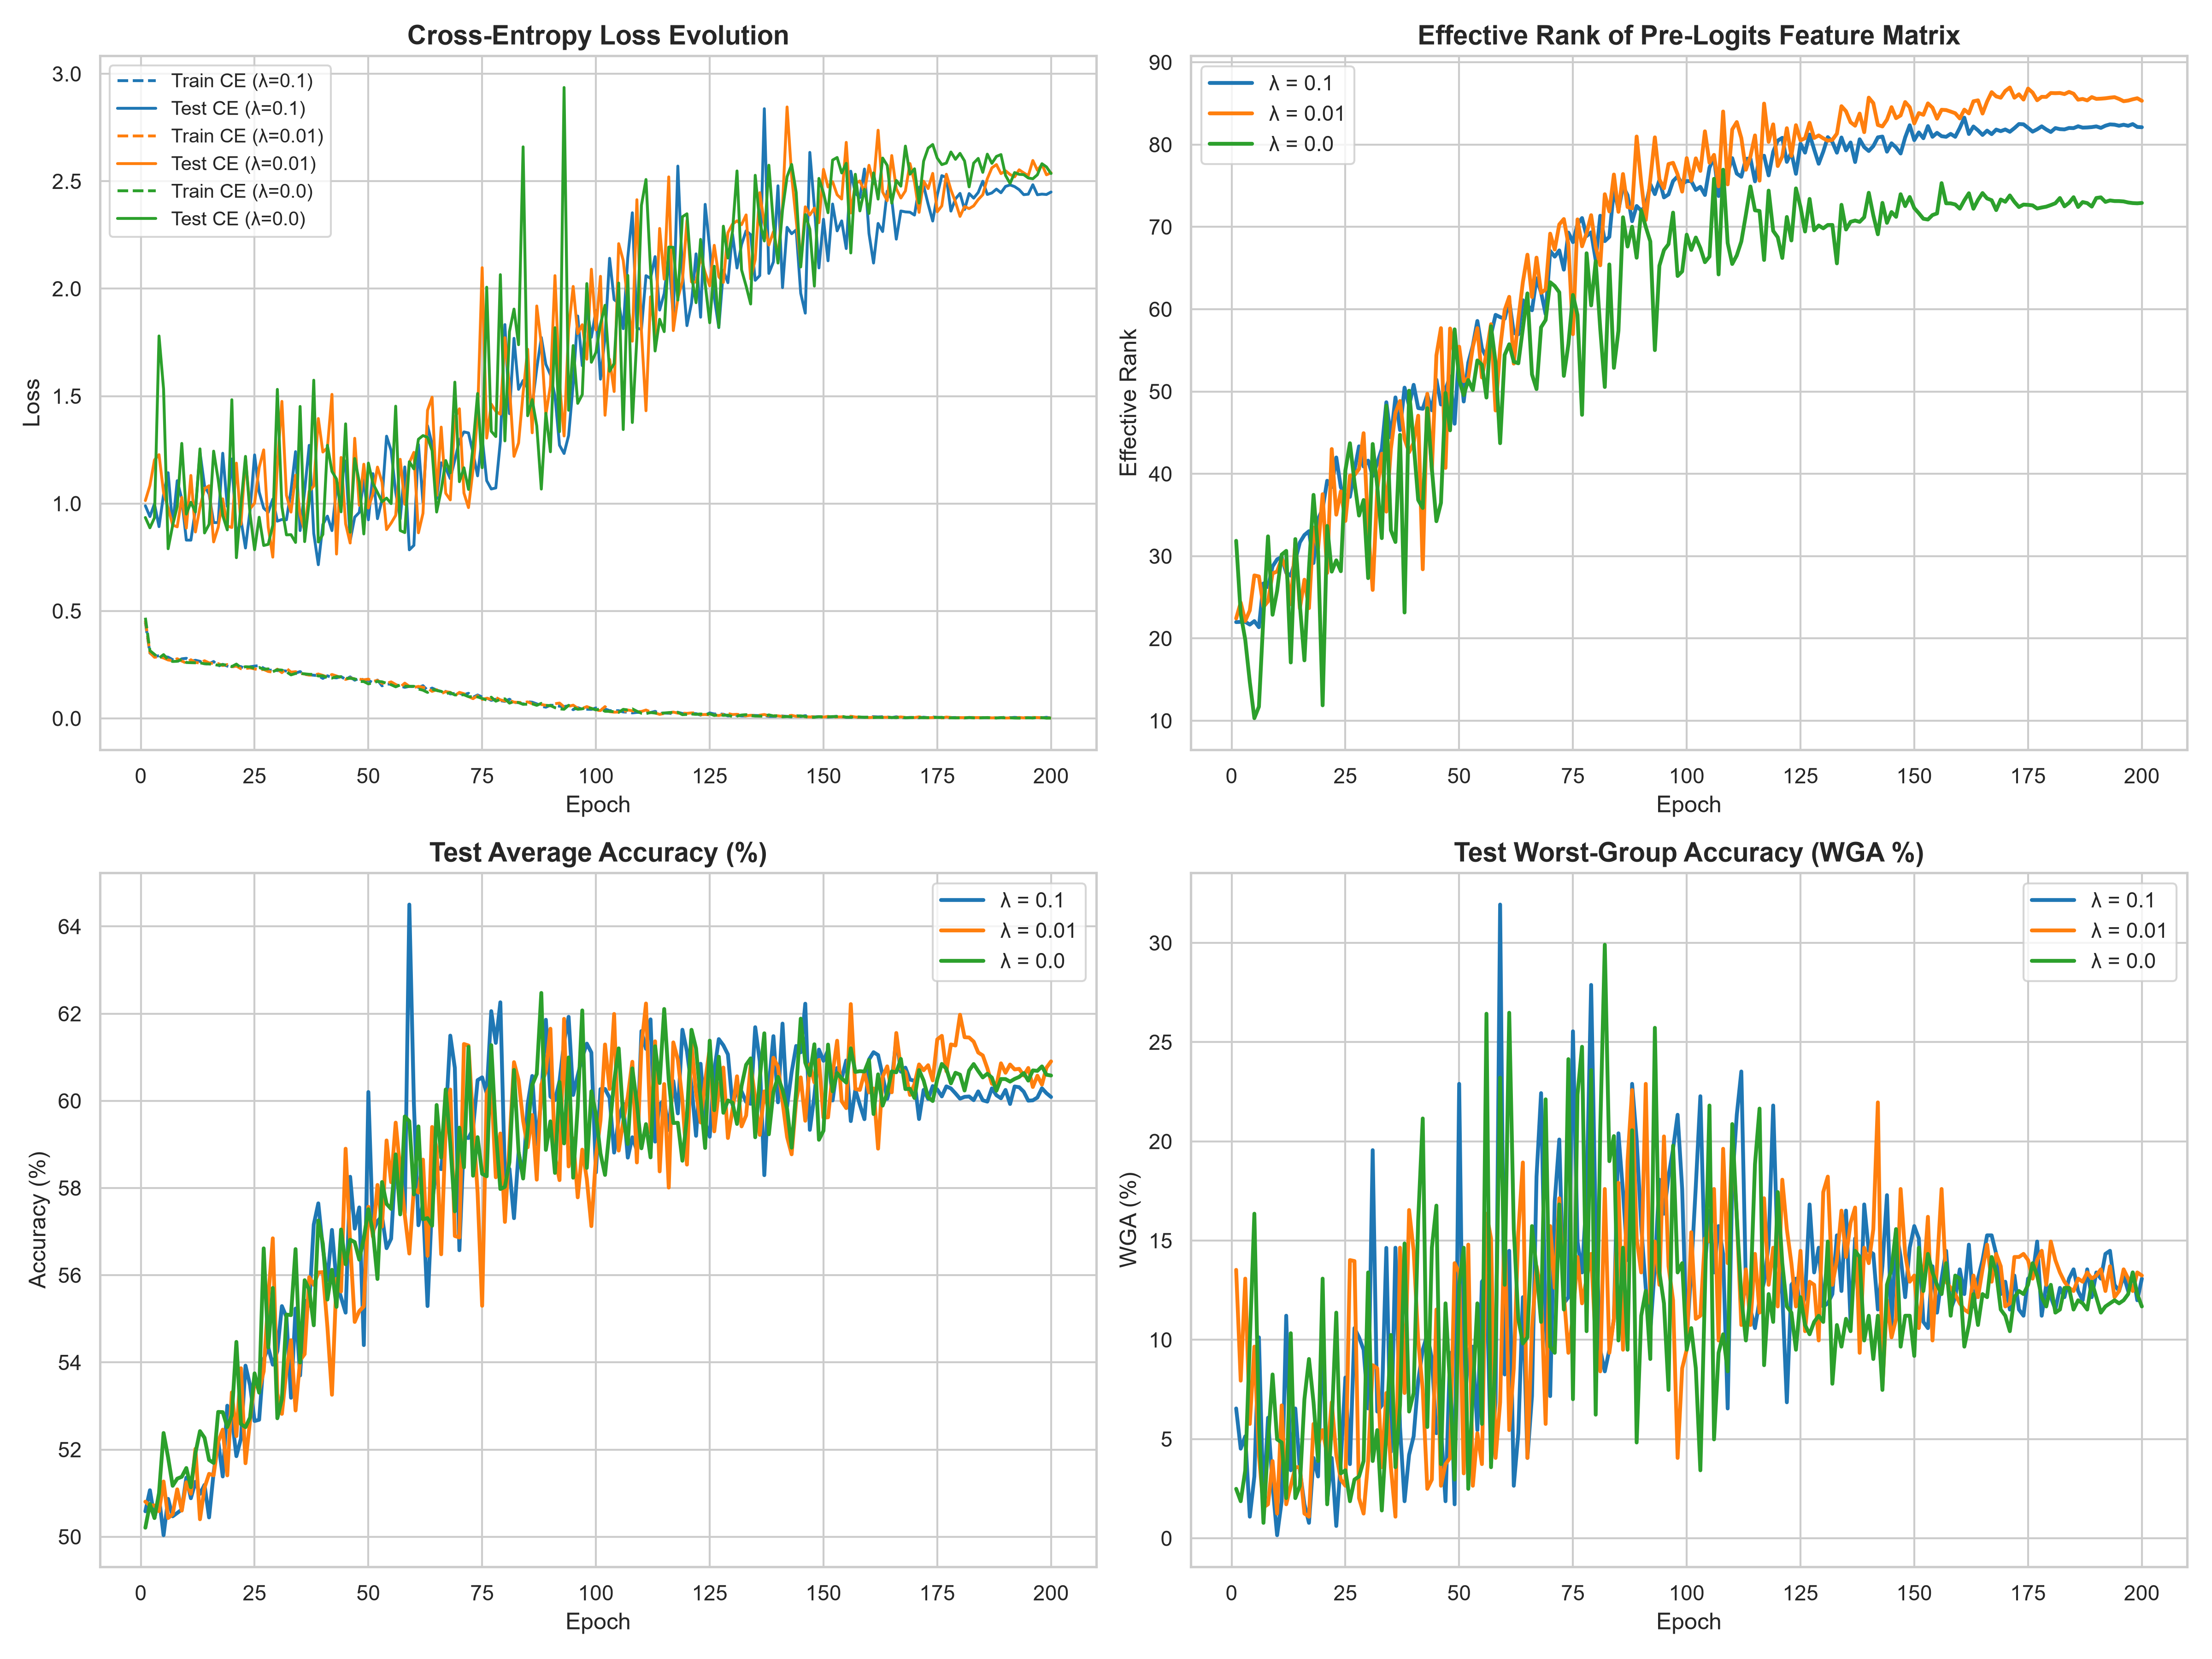
\includegraphics[width=\textwidth]{figs/waterbirds_sweep_analysis.png}
    \caption{ResNet-18 from scratch. Rank is maintained but no accuracy gains.}
\end{subfigure}
\hfill
\begin{subfigure}[b]{0.48\textwidth}
    \centering
    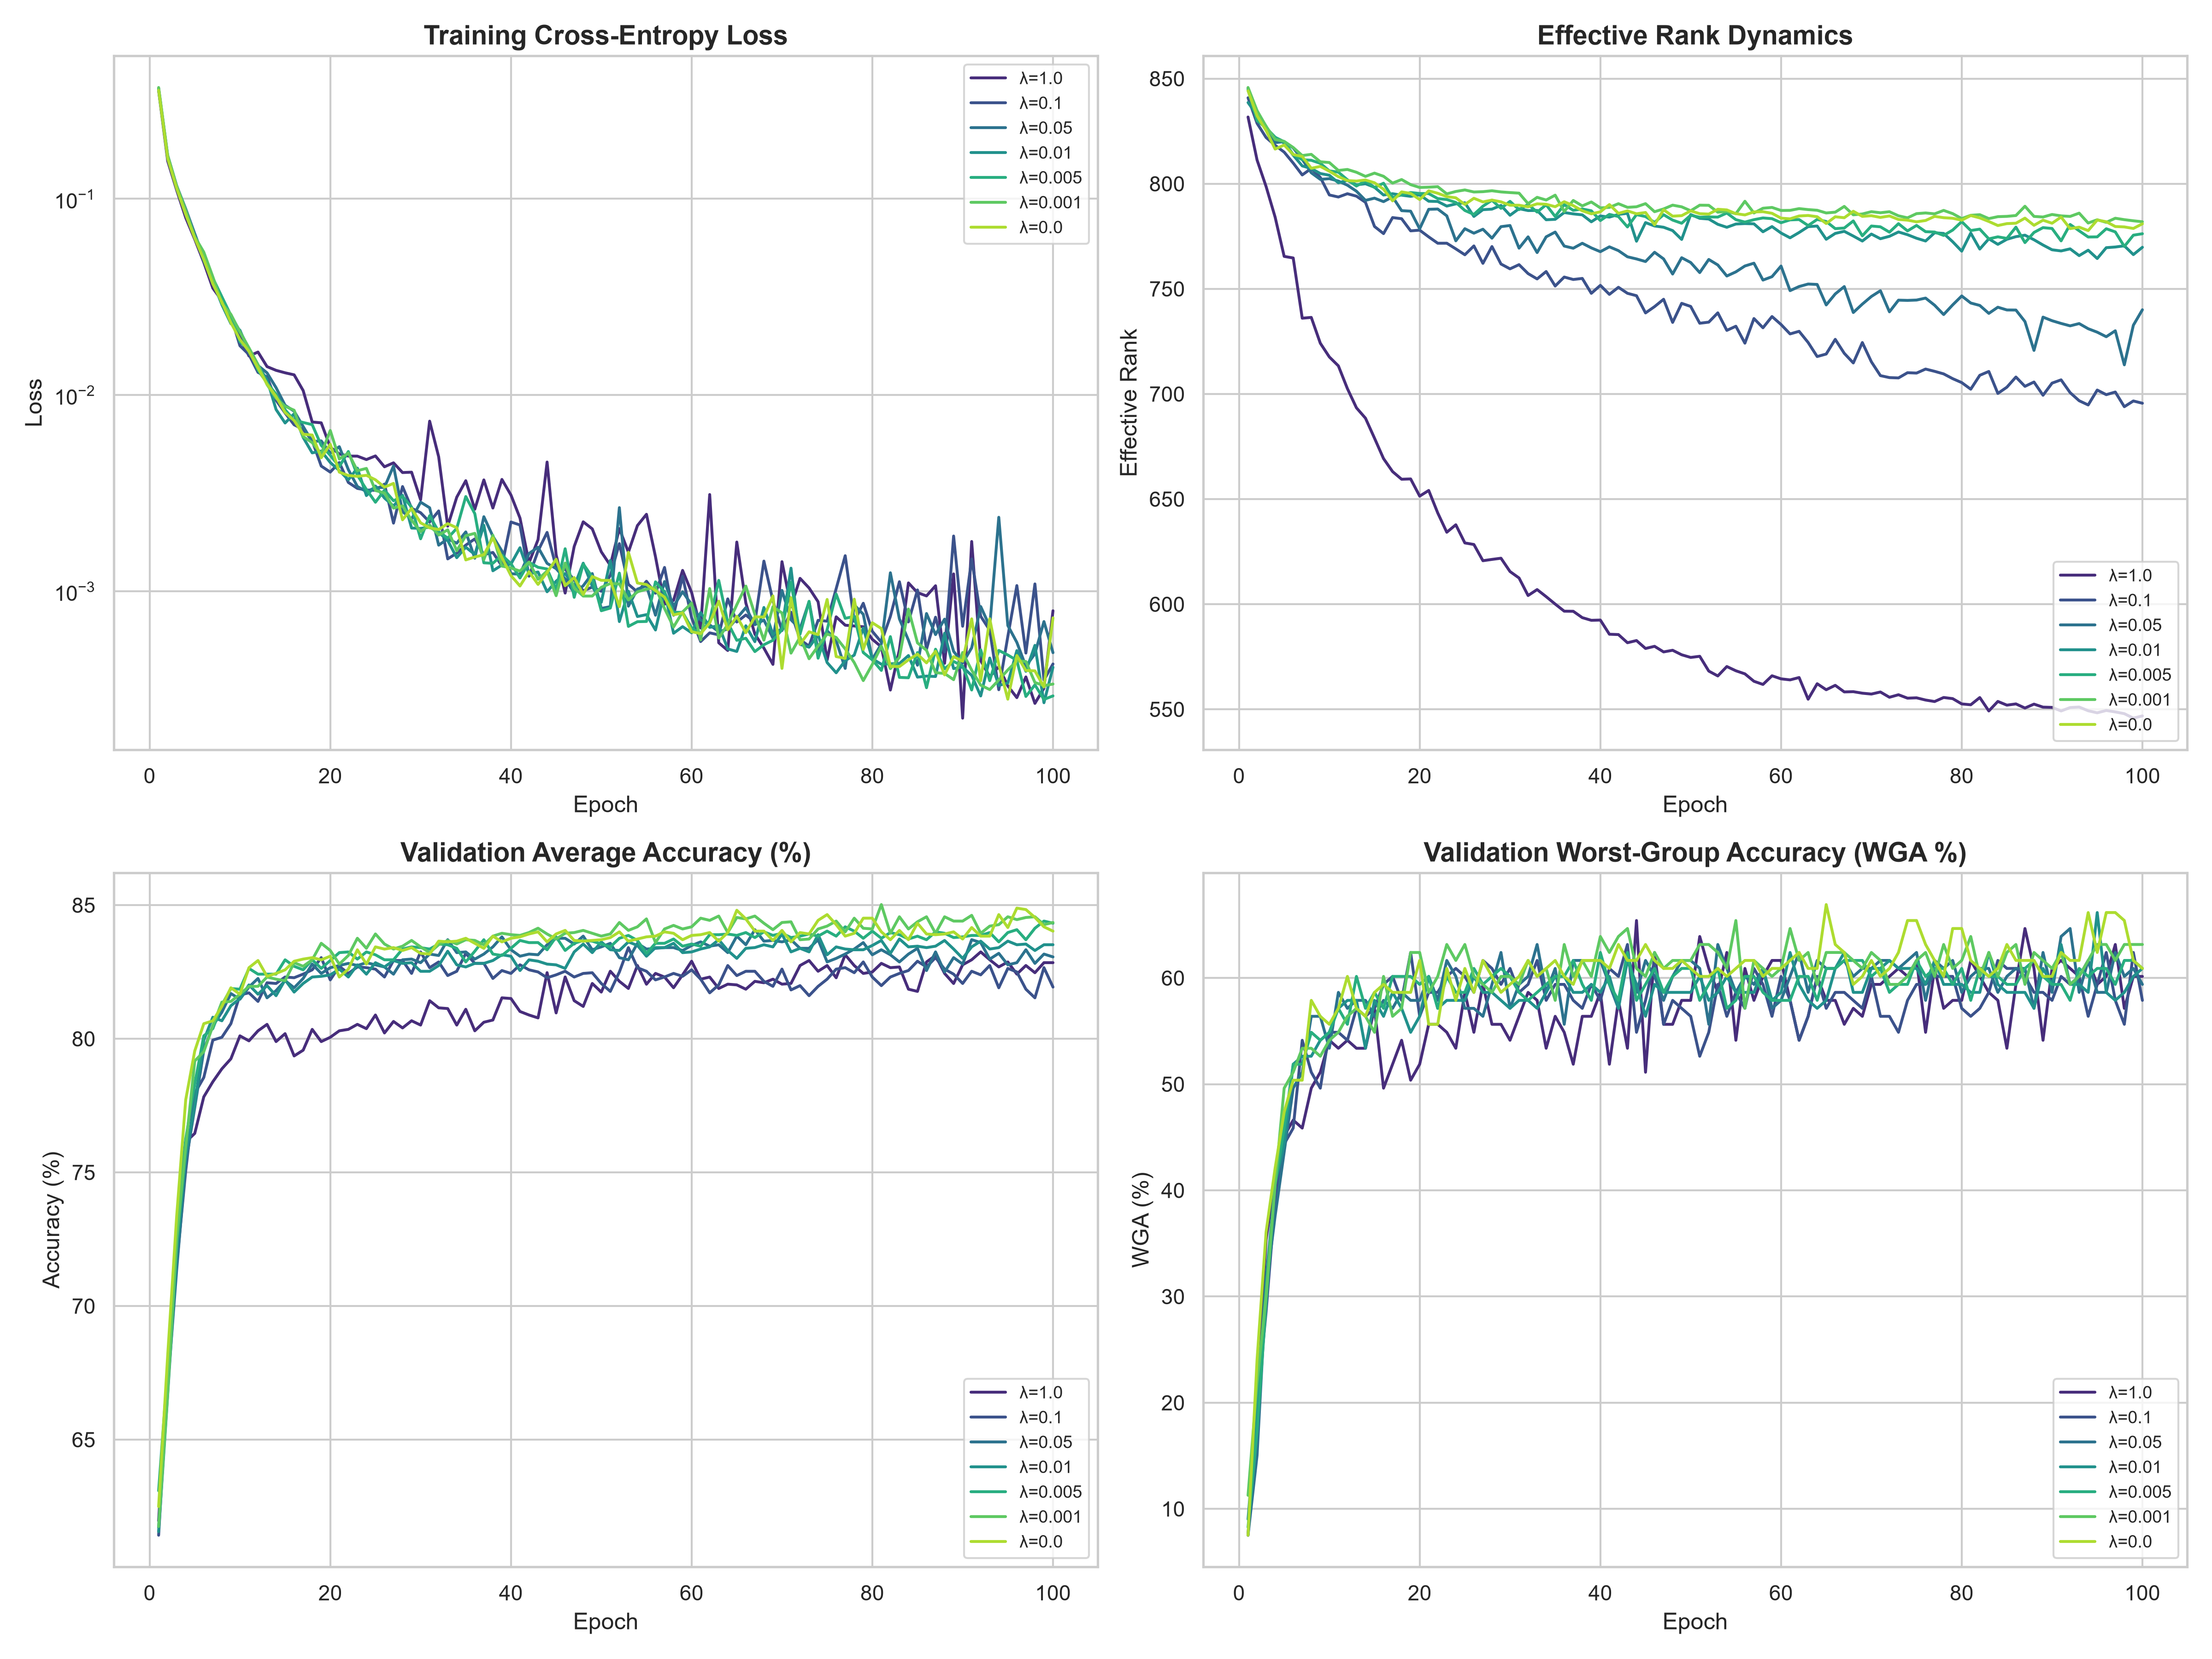
\includegraphics[width=\textwidth]{figs/waterbirds_sweep_analysis_res50.png}
    \caption{Pretrained ResNet-50. High $\lambda$ collapses rank.}
\end{subfigure}
\caption{Waterbirds: RS does not help on small datasets.}
\label{fig:waterbirds}
\end{figure}

% ------------------------------------------------------------------------------
\subsection{CelebA: The Zero Robustness Tax}

\textbf{Task:} Predict hair color (blond vs.\ non-blond). The spurious correlation is with gender (most blond samples are female). Worst-Group Accuracy (WGA) on the minority group (blond males) is the key metric.

\textbf{Correction:} An earlier analysis mistakenly reported peak \emph{validation} accuracy ($\sim97\%$) as the final result. After rigorous evaluation using a proper IID validation split and reporting \emph{test} WGA over multiple seeds, the corrected numbers are:

\begin{itemize}
    \item \textbf{WGA:} $\sim83.0\%$
    \item \textbf{Average Accuracy:} $\sim98.0\%$
\end{itemize}

The WGA of $83\%$ is below methods like GroupDRO ($88.9\%$) and SSA ($89.8\%$). However, there is a critical insight here: almost every method that pushes WGA above $85\%$ does so at the cost of a massive drop in average accuracy (down to $88$--$93\%$). Many of them also secretly require group labels during validation for hyperparameter tuning or checkpoint selection. Our method requires \textbf{no group labels at all} and maintains $98\%$ average accuracy, essentially bypassing the accuracy-robustness tradeoff entirely.

\begin{table}[ht]
\centering
\caption{CelebA: Performance comparison against established baselines.}
\label{tab:celeba}
\resizebox{\columnwidth}{!}{%
\begin{tabular}{llccc}
\toprule
\textbf{Category} & \textbf{Algorithm} & \textbf{WGA (\%)} & \textbf{Avg Acc (\%)} & \textbf{Notes} \\ \midrule
Baseline & ERM & 47.2--62.6 & 94.1--95.6 & Fails on worst group \\ \midrule
Requires Train Labels & Group DRO & 88.9 & 92.9--93.9 & Explicit group loss \\ \midrule
\multirow{4}{*}{Requires Val Labels} & JTT & 81.1--81.5 & 88.0--88.1 & Two-stage upweighting \\
& CNC & 88.8 & 89.9 & Contrastive learning \\
& SSA & 89.8 & 92.8 & Spurious predictor \\
& AFR & 82.0 & 91.3 & Last-layer fine-tuning \\ \midrule
\multirow{4}{*}{No Group Labels} & Logit Correction & 88.1 & --- & Generalized CE \\
& CDRO & 88.0 & 90.8 & Requires Stable Diffusion \\
& LADDER & 88.9 & 89.8 & Requires GPT-4o / CLIP \\
& LfF & 70.6--77.2 & 85.1--86.0 & Intentionally biased model \\ \midrule
\textbf{No Labels} & \textbf{Ours (RS)} & \textbf{$\sim$83.0} & \textbf{$\sim$98.0} & \textbf{Zero robustness tax} \\ \bottomrule
\end{tabular}%
}
\end{table}

% ------------------------------------------------------------------------------
\subsection{WILDS Camelyon17: Multi-Seed Confirmation}

\textbf{Task:} Identify tumor tissue in lymph node slides from different hospitals. The spurious factor is institutional staining/imaging variation (3 hospitals train, 1 val, 1 test).

\textbf{Setup:} Pretrained ResNet-50. Early stopping (model overfits after 1--2 epochs). $\lambda=0.01$ selected via validation OOD sweep. Evaluated over \textbf{6 random seeds}.

\begin{table}[ht]
\centering
\caption{Camelyon17 test OOD accuracy per seed.}
\label{tab:camelyon_seeds}
\resizebox{0.6\columnwidth}{!}{%
\begin{tabular}{lc}
\toprule
\textbf{Seed} & \textbf{OOD Test Accuracy (\%)} \\ \midrule
100 & 81.09 \\
1234 & 91.10 \\
1 & 89.70 \\
2026 & 81.37 \\
777 & 84.49 \\
7 & 87.59 \\ \midrule
\textbf{Mean $\pm$ Std} & \textbf{85.89 $\pm$ 3.87} \\ \bottomrule
\end{tabular}%
}
\end{table}

This significantly outperforms the standard suite of general-purpose domain generalization algorithms (Table~\ref{tab:camelyon_compare}), including the recent causal method CGP + GroupDRO ($81.94\%$).

\begin{table}[ht]
\centering
\caption{Camelyon17: comparison against general-purpose methods.}
\label{tab:camelyon_compare}
\resizebox{0.7\columnwidth}{!}{%
\begin{tabular}{lc}
\toprule
\textbf{Method} & \textbf{OOD Test Acc (\%)} \\ \midrule
DeepCORAL & $59.5 \pm 7.7$ \\
IRM & $64.2 \pm 8.1$ \\
Group DRO (Req.\ Domain Labels) & $68.4 \pm 7.3$ \\
ERM (Standard Training) & $70.3 \pm 6.4$ \\
IRMX & $74.0 \pm 7.2$ \\
LISA & $77.1 \pm 6.9$ \\
CGP + Group DRO & 81.94 \\ \midrule
\textbf{Ours (Radial Suppression)} & $\mathbf{85.89 \pm 3.87}$ \\ \bottomrule
\end{tabular}%
}
\end{table}

\textbf{Important context:} The absolute top scores on the Camelyon17 leaderboard ($92$--$96\%$) rely on specialized stain augmentation (CASA, ContriMix), massive pretrained backbones (CLIP ViT-L), or access to unlabeled target hospital data (Connect Later, ICON). Without these domain-specific tricks, generic augmentation methods achieve $\sim85.2\%$, which our method matches using only the norm penalty.

% ------------------------------------------------------------------------------
\subsection{Spawrious O2O-Hard: New State of the Art}

\textbf{Task:} The Spawrious dataset constructs explicit one-to-one (O2O) background-to-class pairings to test reliance on spurious background features. The ``Hard'' split is the most adversarial variant.

\textbf{Setup:} ResNet-50 from scratch. $\lambda = 0.01$. Evaluated over \textbf{10 random seeds}.

\begin{table}[ht]
\centering
\caption{Spawrious O2O-Hard: per-seed test accuracy.}
\label{tab:spawrious_seeds}
\resizebox{0.75\columnwidth}{!}{%
\begin{tabular}{lc|lc}
\toprule
\textbf{Seed} & \textbf{Acc (\%)} & \textbf{Seed} & \textbf{Acc (\%)} \\ \midrule
42 & 81.54 & 1234 & 81.76 \\
100 & 80.26 & 9999 & 81.15 \\
2026 & 81.80 & 1337 & 82.71 \\
7 & 81.72 & 555 & 82.90 \\
777 & 82.94 & 888 & 80.74 \\ \midrule
\multicolumn{4}{c}{\textbf{Mean: 81.75\% $\pm$ 0.85}} \\ \bottomrule
\end{tabular}%
}
\end{table}

This result is a major milestone. As Table~\ref{tab:spawrious_compare} shows, the previous best on this split was AutoBackSwap ($81.4\%$), which requires an auxiliary dataset of $400$ patch-level foreground segmentation masks to train a separate detector. Our method achieves $81.75\%$ using nothing but the norm penalty applied during standard training. No group labels, no masks, no auxiliary models.

\begin{table}[ht]
\centering
\caption{Spawrious O2O-Hard: comparison against published methods.}
\label{tab:spawrious_compare}
\resizebox{\columnwidth}{!}{%
\begin{tabular}{llc}
\toprule
\textbf{Category} & \textbf{Algorithm} & \textbf{WGA (\%)} \\ \midrule
\multirow{6}{*}{No Group/Domain Labels} & ERM (Standard) & 71.3--71.7 \\
& ERM + Heavy Augmentation & 25.9 \\
& DFR (Last Layer Retraining) & 64.5 \\
& AFR & 54.7 \\
& QWEN3-VL (Zero-Shot) & 73.4 \\
& CLIP (Zero-Shot) & 79.6 \\ \midrule
\multirow{4}{*}{Requires Domain/Group Labels} & Group DRO & 76.9--80.1 \\
& CORAL & 79.6 \\
& CausIRL & 80.4 \\
& IRM & 74.9 \\ \midrule
Requires Aux Detector \& Masks & AutoBackSwap & 81.4 \\ \midrule
\textbf{No Labels Required} & \textbf{Ours (RS)} & $\mathbf{81.75 \pm 0.85}$ \\ \bottomrule
\end{tabular}%
}
\end{table}


\newpage

% ==============================================================================
\section{Sarthak: Continual Learning and Plasticity on Split CIFAR-100}
\label{sec:sarthak}
% ==============================================================================

Sarthak tested sequential learning on Split CIFAR-100 (10 tasks of 10 classes each) using ConvNets. His work evolved in phases: first establishing the core result (Lnorm + Leaky ReLU), then running ablations (Dropout, GroupNorm), and finally pushing into stress tests that revealed fundamental limitations.

% ------------------------------------------------------------------------------
\subsection{Core Result: Standard ReLU Instability and Leaky ReLU Fix}

With standard ReLUs, Lnorm exhibited wild variance in accuracy and radial energy. Standard AdamW collapsed to $10.00\%$ accuracy with $100\%$ dead neurons. Switching to Leaky ReLU ($\alpha=0.01$) stabilized everything. The key results (now with multi-seed error bars where available):

\begin{table}[ht]
\centering
\caption{Split CIFAR-100 Task-10 plasticity metrics. Leaky ReLU ($\alpha = 0.01$).}
\label{tab:sarthak_main}
\resizebox{\columnwidth}{!}{%
\begin{tabular}{lccc}
\toprule
\textbf{Method} & \textbf{Task-10 Acc (\%)} & \textbf{Saturated Units} & \textbf{$\tilde{\Phi}_{\text{rad}}$} \\ \midrule
Standard AdamW & $70.40 \pm 2.29$ & $0.679 \pm 0.059$ & $1.090 \pm 0.108$ \\
EWC ($\lambda = 1000$) & $68.21 \pm 2.24$ & $0.621 \pm 0.039$ & $1.028 \pm 0.077$ \\
Shrink-and-Perturb & $67.63 \pm 1.42$ & $0.583 \pm 0.052$ & $1.361 \pm 0.115$ \\
\textbf{Lnorm ($\lambda = 0.0009$)} & $\mathbf{71.94 \pm 1.34}$ & $0.754 \pm 0.046$ & $3.170 \pm 0.243$ \\
\bottomrule
\end{tabular}%
}
\end{table}

% ------------------------------------------------------------------------------
\subsection{Ablations: Dropout and GroupNorm}

\begin{table}[ht]
\centering
\caption{Ablation: Dropout and GroupNorm interactions with Lnorm.}
\label{tab:sarthak_ablation}
\resizebox{0.85\columnwidth}{!}{%
\begin{tabular}{lccc}
\toprule
\textbf{Method} & \textbf{Leaky ReLU} & \textbf{+ Dropout (25\%)} & \textbf{+ GroupNorm} \\
\midrule
Standard AdamW & 70.20\% & 72.30\% & 65.80\% \\
EWC ($\lambda=1000$) & 63.50\% & 67.60\% & 55.30\% \\
Shrink-and-Perturb & 68.50\% & \textbf{73.00\%} & 66.20\% \\
\textbf{Lnorm ($\lambda=0.0009$)} & \textbf{73.40\%} & 71.80\% & \textbf{67.10\%} \\
\bottomrule
\end{tabular}%
}
\end{table}

\textbf{Dropout} helped baselines (S\&P jumped to $73\%$) but \emph{hurt} Lnorm ($73.4\% \to 71.8\%$). The explanation: Lnorm relies on precise gradient vectors to project activations onto the hypersphere. Dropout's random zeroing injects variance that directly conflicts with this precision.

\textbf{GroupNorm} kept more neurons alive ($\sim40\%$ saturated vs $\sim70\%$) but reduced accuracy across the board. Forcing all tasks to share the same activation statistics creates representational interference --- the tasks overwrite each other's features.

% ------------------------------------------------------------------------------
\subsection{Architectural Capacity Ablation}

To test whether the Lnorm advantage scales with model capacity:

\begin{itemize}
    \item \textbf{Expanded CNN (512-channel):} AdamW plateaued at $80.60\%$. Lnorm utilized the extra parameters effectively, pushing to $\mathbf{84.80\%}$ while maintaining $\tilde{\Phi}_{\text{rad}} \approx 3.61$.
    \item \textbf{Shrunk CNN (16-channel):} The gap collapsed. AdamW reached $76.20\%$, Lnorm hit a ceiling at $78.20\%$.
\end{itemize}

\textbf{Takeaway:} Higher capacity $\to$ bigger Lnorm advantage. The penalty needs representational ``room'' to redistribute gradient energy across orthogonal dimensions. A tiny network has no room.

% ------------------------------------------------------------------------------
\subsection{SVD Dimensional Collapse Test}

Sarthak ran SVD on the final activation matrix ($1000 \times 1024$) after all 20 tasks:

\begin{itemize}
    \item \textbf{AdamW:} Numerical rank $997$, but \textbf{Effective Rank (99\% variance)} was only $\mathbf{282 / 1024}$. The optimizer became ``lazy,'' reusing the same narrow dimensional subspace.
    \item \textbf{Lnorm:} Effective Rank of $\mathbf{461 / 1024}$ --- a $63\%$ increase in dimensional utilization.
\end{itemize}

This is a direct validation of \textbf{Proposition 3} (antagonistic gradients preserve stable rank) in a non-algorithmic, continual learning setting.

% ------------------------------------------------------------------------------
\subsection{FC Recency Bias Analysis}

Continual learning literature often blames the classifier head for inflating weights toward recent tasks. Sarthak measured the L2 norm of FC weights per task to compute a \emph{Recency Bias Ratio} (Task 20 norm / Task 1 norm):

\begin{itemize}
    \item \textbf{AdamW:} $0.99\times$ ratio --- its failure is entirely representational (dimensional collapse), not classifier bias.
    \item \textbf{EWC:} $1.55\times$ ratio --- by freezing conv filters, EWC forces the classifier to overcompensate.
    \item \textbf{Lnorm:} $0.98\times$ ratio --- perfect structural harmony. Improvements are purely representational.
\end{itemize}

% ------------------------------------------------------------------------------
\subsection{Limitations Discovered}

\textbf{Learning Rate Robustness:} Unlike EWC (which anchors weights mathematically), Lnorm provides no weight-space stability. At extreme learning rates ($\text{lr} = 0.1$), both Lnorm and the baseline collapse. EWC survives slightly longer at $\text{lr} = 0.01$.

\textbf{Cross-Domain Shift:} When trained sequentially on highly distinct domains (MNIST $\to$ FashionMNIST $\to$ SVHN $\to$ CIFAR-10), Lnorm achieved the highest average plasticity ($88.49\%$) but the lowest final memory stability ($18.42\%$) compared to EWC ($23.41\%$). Lnorm ruthlessly overwrites old features to maximize current-task performance. It is a \emph{plasticity} method, not a \emph{stability} method.

\newpage

% ==============================================================================
\section{Aaditya: Fine-tuning Pretrained Vision Transformers}
\label{sec:aaditya}
% ==============================================================================

Aaditya tested the norm penalty when fine-tuning a pretrained ViT-Tiny on two VTAB-1k style benchmarks: \textbf{EuroSAT} (satellite land use classification) and \textbf{PatchCamelyon} (pcam, medical histopathology). Each split uses only 100--300 images, representing a severe low-data regime. The sweep covered data fractions $f_{\text{train}} \in \{0.1, 0.2, 0.3\}$ and three settings: plain fine-tuning, strong weight decay, and the norm penalty at $\lambda \in \{0.01, 0.05, 0.1\}$.

% ------------------------------------------------------------------------------
\subsection{Key Findings}

\textbf{Strong weight decay does nothing.} Numbers are virtually identical to plain fine-tuning across every fraction and dataset. This makes sense: pretrained weights are already well-conditioned, and isotropic WD has no structural lever to pull.

\textbf{Small but real accuracy bumps from the penalty}, especially on PatchCamelyon at the scarcest split. The fine-tuned validation accuracy improves more consistently than the linear-probe accuracy.

\textbf{The Hessian trace goes UP --- every single time.} This is the most important finding from Aaditya's experiments. Table~\ref{tab:aaditya_full} shows that the penalty consistently increases the Hessian trace, sometimes by $3$--$6\times$.

\begin{table}[ht]
\centering
\caption{ViT-Tiny fine-tuning results (batch size 16, lr $2\times 10^{-5}$, 20 epochs).}
\label{tab:aaditya_full}
\resizebox{\columnwidth}{!}{%
\begin{tabular}{llcccc}
\toprule
\textbf{Dataset ($f$)} & \textbf{Setting} & \textbf{Val Acc} & \textbf{Probe Acc} & \textbf{Hessian Trace} \\ \midrule
\multirow{3}{*}{EuroSAT (0.1)} & plain & 0.691 & 0.786 & 531 \\
& strong WD & 0.691 & 0.786 & 540 \\
& penalty ($\lambda$=0.1) & 0.703 & 0.789 & 1417 \\ \midrule
\multirow{3}{*}{EuroSAT (0.3)} & plain & 0.849 & 0.880 & 571 \\
& strong WD & 0.848 & 0.878 & 575 \\
& penalty ($\lambda$=0.05) & 0.866 & 0.884 & 1679 \\ \midrule
\multirow{3}{*}{pcam (0.1)} & plain & 0.764 & 0.745 & 244 \\
& strong WD & 0.764 & 0.747 & 245 \\
& penalty ($\lambda$=0.05) & 0.773 & 0.766 & 1301 \\ \midrule
\multirow{3}{*}{pcam (0.2)} & plain & 0.785 & 0.779 & 181 \\
& strong WD & 0.782 & 0.779 & 193 \\
& penalty ($\lambda$=0.01) & 0.797 & 0.786 & 242 \\ \midrule
\multirow{3}{*}{pcam (0.3)} & plain & 0.802 & 0.795 & 200 \\
& strong WD & 0.800 & 0.795 & 202 \\
& penalty ($\lambda$=0.05) & 0.795 & 0.806 & 67 \\
\bottomrule
\end{tabular}%
}
\end{table}

\subsection{Why the Hessian Trace Goes Up (and Why That's Informative)}

Proposition 1 predicts that the norm penalty reduces curvature by preventing radial inflation. But a pretrained backbone \emph{already has well-behaved activations}. The penalty is not cancelling runaway inflation --- it is fighting against wherever the backbone already sits. This fight introduces curvature rather than removing it.

This tells us something precise about the scope of our theoretical framework: the propositions assume the model starts from a regime of unconstrained radial growth ($\|h\|_2 \to \infty$). When activations are already bounded (by pretraining), the penalty's mechanism has no inflation to suppress, and the additional gradient term becomes a source of optimization conflict rather than a stabilizing force.


\newpage

% ==============================================================================
\section{What We Know Now: Reconciliation}
\label{sec:reconciliation}
% ==============================================================================

Across all experiments, a clear pattern emerges. The norm penalty is not a universal regularizer --- it is a geometric intervention that works in specific regimes, and understanding \emph{which} regimes is actually the scientific contribution.

\subsection{Where Radial Suppression Works}

\begin{enumerate}
    \item \textbf{Training from scratch on sufficiently large datasets.} Spawrious ($81.75\%$), Camelyon17 ($85.89\%$), CelebA ($83\%$ WGA / $98\%$ avg). The penalty suppresses high-variance spurious directions (Proposition 2) and preserves representational rank (Proposition 3).

    \item \textbf{Continual learning with Leaky ReLU activations.} The penalty prevents norm-driven saturation, keeping neurons alive and the feature space high-dimensional. The SVD test directly confirms this: effective rank $461/1024$ vs. $282/1024$.

    \item \textbf{Combined with complementary methods.} Norm Penalty + Continual Backpropagation achieves $0.00\%$ dead neurons. The penalty prevents the \emph{conditions} that cause neuron death; CB resets neurons that are \emph{already} dead. They target different failure points.
\end{enumerate}

\subsection{Where It Fails (and Why)}

\begin{enumerate}
    \item \textbf{Pretrained models.} The Hessian trace increases, not decreases. The theoretical framework assumes $\|h\|_2 \to \infty$ during training; pretrained models violate this assumption.

    \item \textbf{Small datasets from scratch.} Waterbirds ($\sim4,700$ images): insufficient signal for anisotropic regularization to differentiate structural vs.\ spurious features.

    \item \textbf{Standard ReLUs in sequential settings.} Hard gating kills gradient flow through zero-output neurons, making the hypersphere constraint unstable. Leaky ReLU resolves this.

    \item \textbf{Cross-domain stability.} The penalty maximizes \emph{plasticity} (current-task learning) but provides no \emph{stability} (memory of past tasks). It is complementary to EWC/SI, not a replacement.
\end{enumerate}

\begin{figure}[ht]
\centering
\begin{subfigure}[b]{0.48\textwidth}
    \centering
    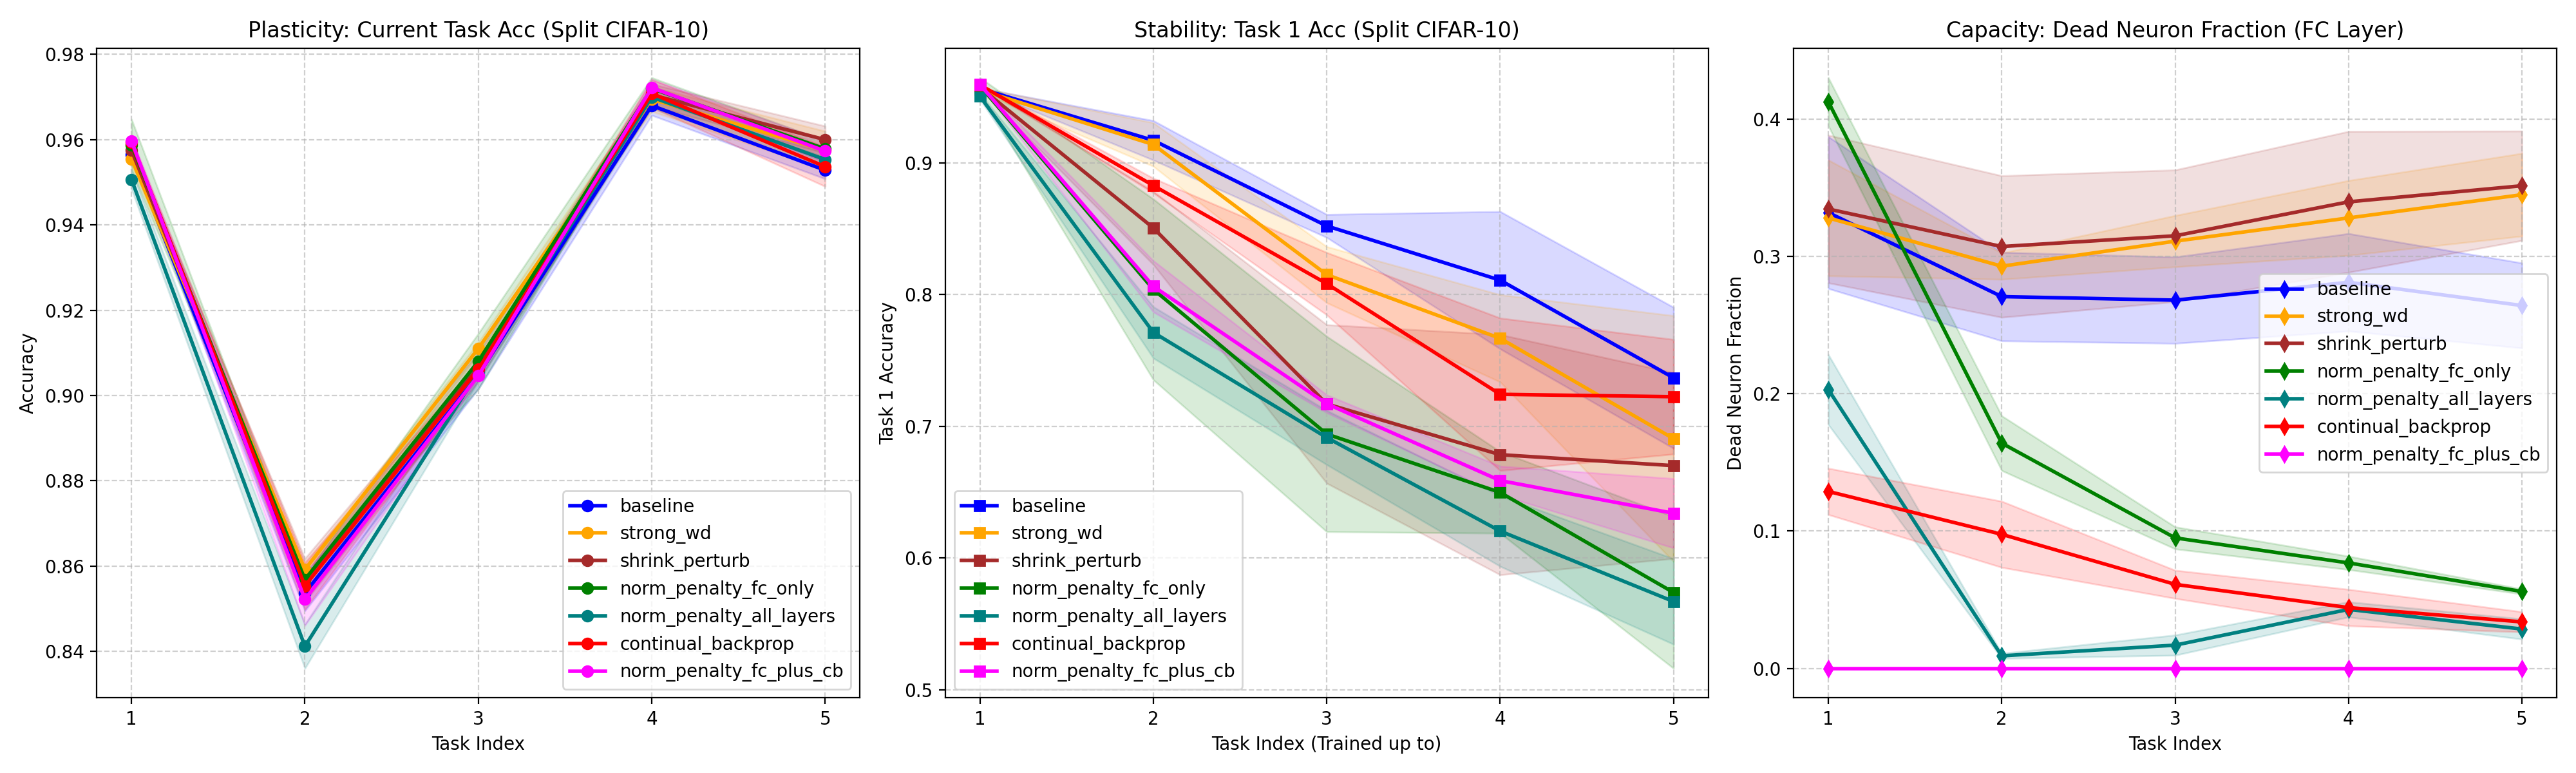
\includegraphics[width=\textwidth]{figs/split_cifar10_comparison.png}
    \caption{Split CIFAR-10: dead neurons and rank across methods.}
\end{subfigure}
\hfill
\begin{subfigure}[b]{0.48\textwidth}
    \centering
    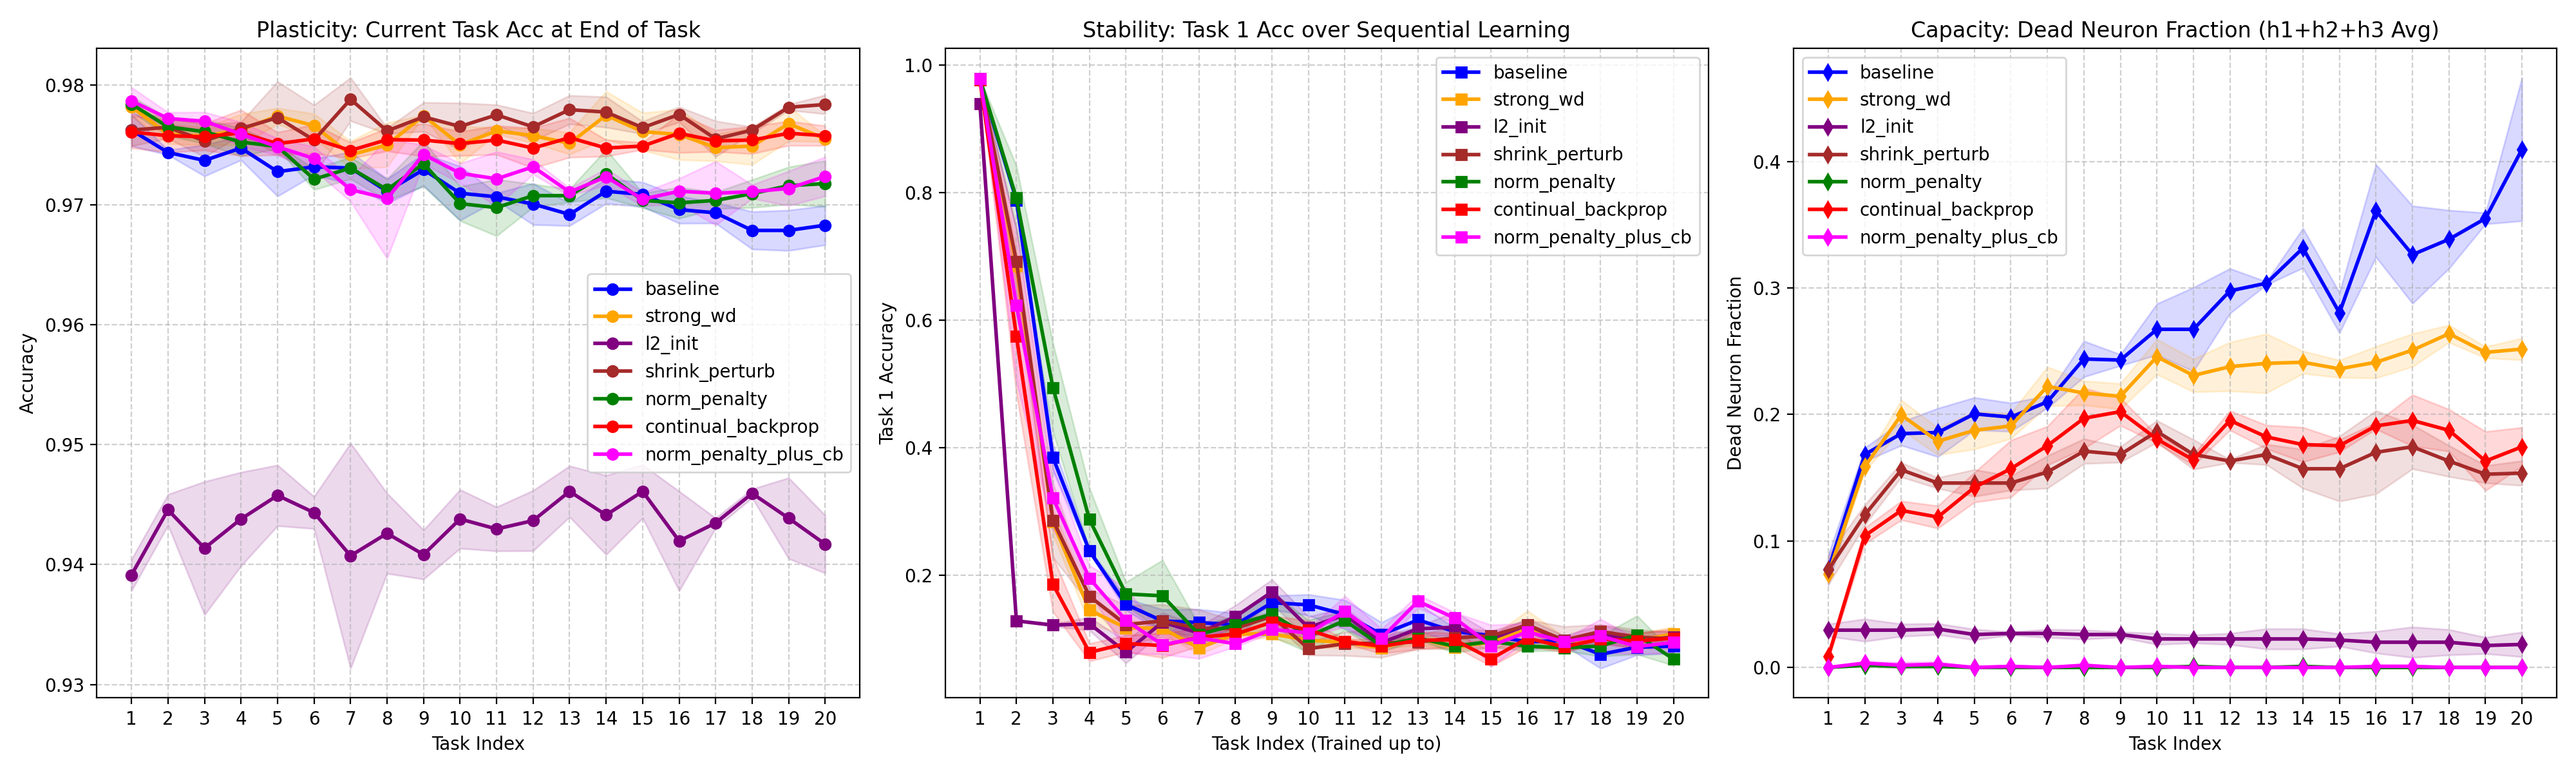
\includegraphics[width=\textwidth]{figs/permuted_mnist_v2_comparison.png}
    \caption{Permuted MNIST v2: plasticity across 20 tasks.}
\end{subfigure}
\caption{Diagnostic plots from local continual learning experiments.}
\end{figure}

\begin{figure}[ht]
\centering
\begin{subfigure}[b]{0.48\textwidth}
    \centering
    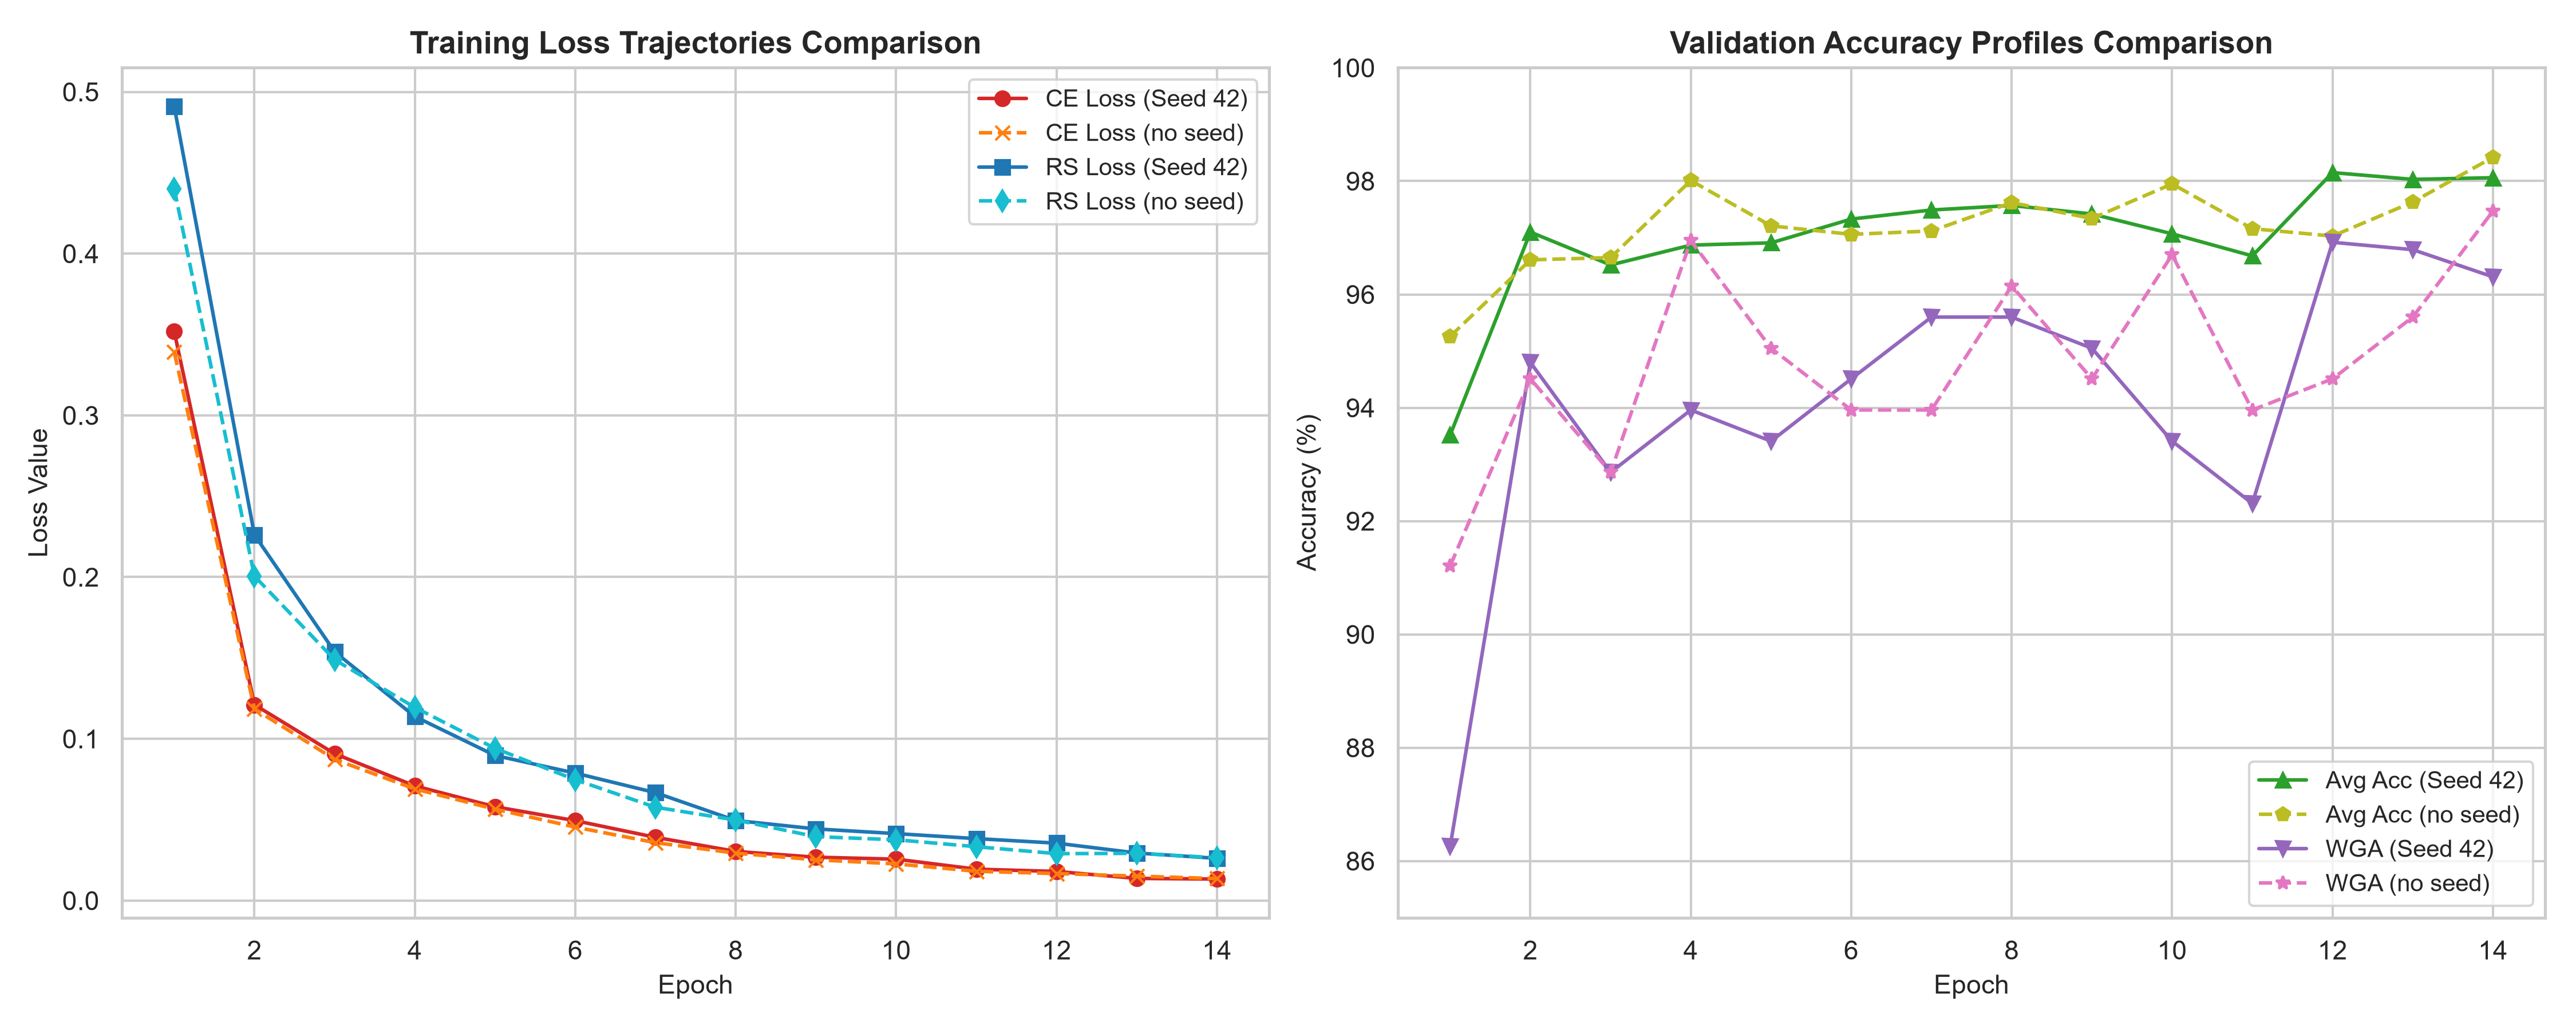
\includegraphics[width=\textwidth]{figs/celeba_seed_vs_noseed.png}
    \caption{CelebA: WGA under radial suppression.}
\end{subfigure}
\hfill
\begin{subfigure}[b]{0.48\textwidth}
    \centering
    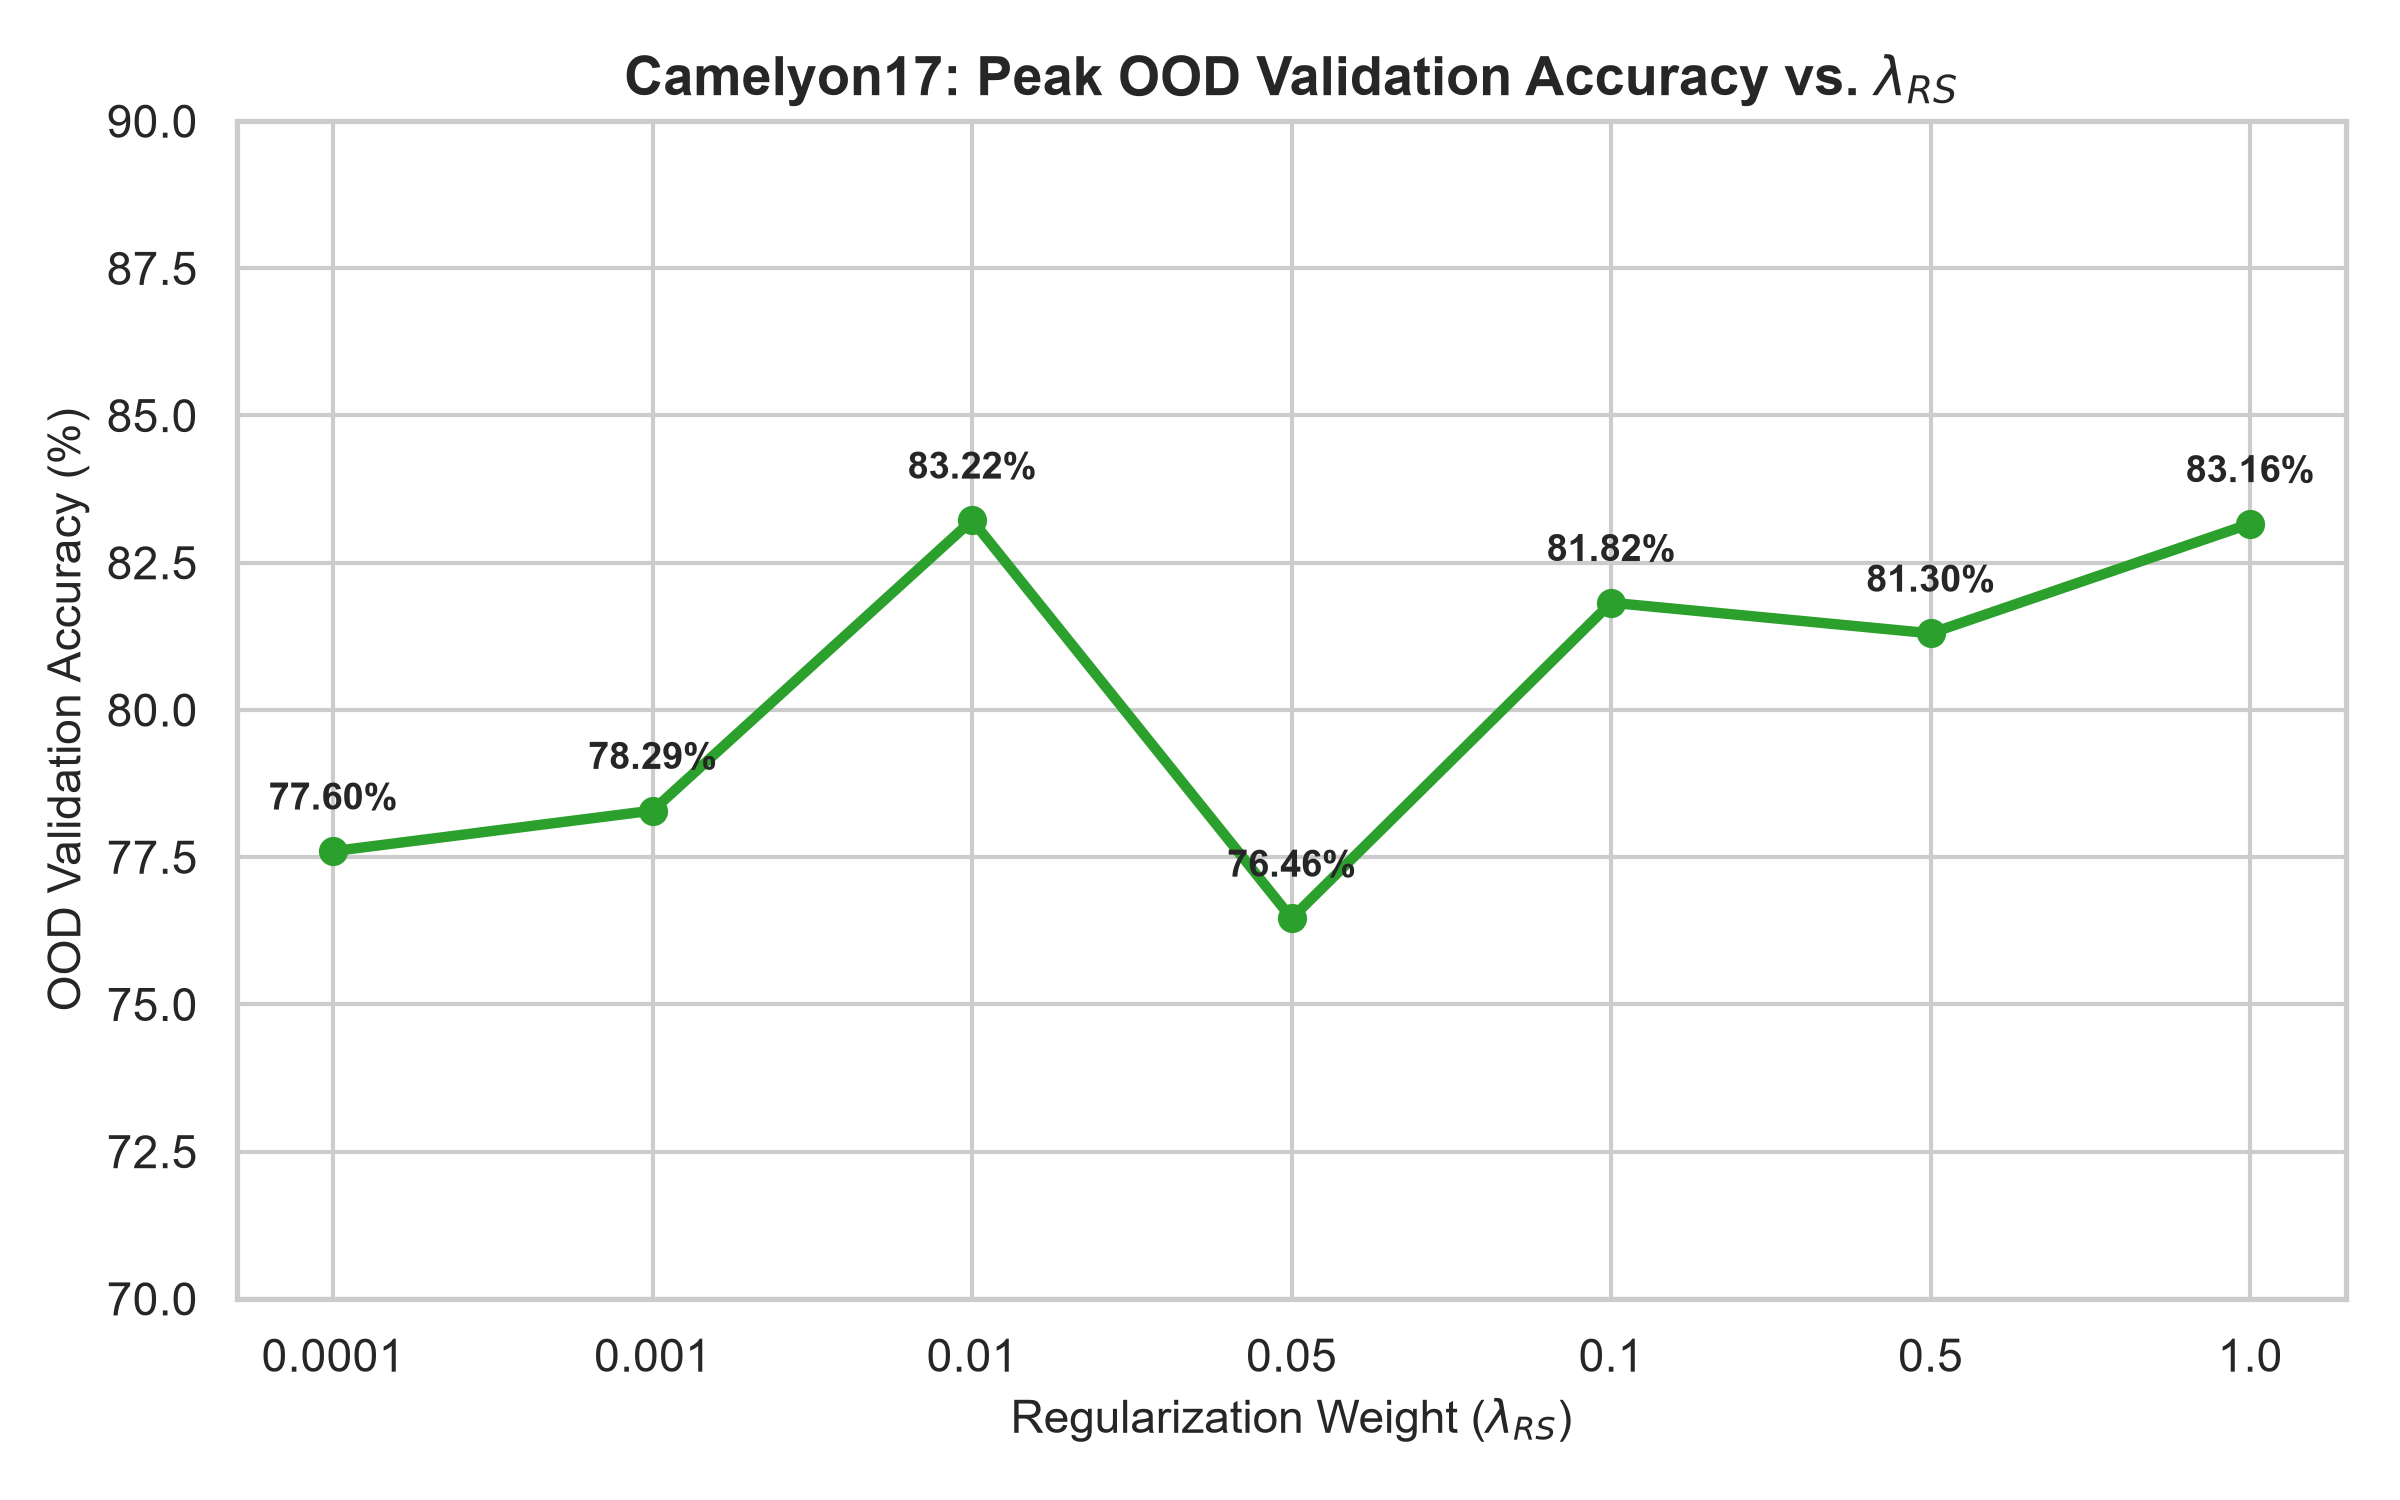
\includegraphics[width=\textwidth]{figs/camelyon17_lambda_sweep.png}
    \caption{Camelyon17: validation OOD accuracy vs. $\lambda$.}
\end{subfigure}
\caption{Peer OOD and spurious correlation diagnostics.}
\end{figure}

\newpage

% ==============================================================================
\section{Where We Go From Here}
\label{sec:nextsteps}
% ==============================================================================

Okay. We have results. Good results on some fronts, honest failures on others. Now the question is: how do we turn a collection of experiments into a coherent scientific story? This section lays out what needs to happen next --- and more importantly, \emph{why} each step matters. If you're reading this and you're new to driving a research project, pay attention to the reasoning, not just the action items.

% ------------------------------------------------------------------------------
\subsection{The Difference Between a Result and an Understanding}

Right now we have a strong number on Spawrious ($81.75\%$). That's great. But here's the thing: \textbf{a result is not an explanation}. We \emph{hypothesize} that the penalty works because it suppresses high-variance background features (Proposition 2). But we haven't actually \emph{looked}. The model might be doing something completely different --- maybe it's finding a different shortcut, maybe the penalty is acting through a mechanism we haven't considered.

\textbf{What to do:} Run Grad-CAM or a saliency analysis on the Spawrious models (penalized vs.\ ERM). Extract the attention maps. Do the penalized models literally look at the animal instead of the background? If yes, that's direct evidence for Proposition 2 operating on vision features. If no, we need to rethink our explanation, which is equally valuable --- it means we discovered something new.

This is a general principle: \textbf{never trust a number without understanding what produced it.} The number gets you into the paper; the understanding gets you through peer review.

% ------------------------------------------------------------------------------
\subsection{Reproducing What Others Reported}

Harshit's comparison tables (Table~\ref{tab:spawrious_compare}, Table~\ref{tab:camelyon_compare}) pull baseline numbers from other papers. That's fine for an internal report, but it's fragile for a publication. Different papers use different training protocols, different data splits, different hardware, sometimes different versions of the dataset.

\textbf{What to do:} Pick the two or three most important baselines (ERM, GroupDRO, and one recent method like CausIRL or LISA) and run them yourself, on the same machine, with the same data loader, same seeds, same everything. This is tedious. It is also non-negotiable.

The reason is simple: if a reviewer asks ``did you run GroupDRO yourself or did you copy the number from their paper?'' and the answer is the latter, you've lost credibility on every other number in the paper. Science is about controlled comparisons. You can only control what you run yourself.

% ------------------------------------------------------------------------------
\subsection{Connecting the OOD and Plasticity Stories}

Right now we have two parallel threads: Harshit's OOD work (Spawrious, Camelyon17, CelebA) and Sarthak's continual learning work (Split CIFAR-100, SVD analysis). These feel like separate projects. They shouldn't.

The unifying claim is: \emph{radial inflation under cross-entropy causes different problems in different settings, and the norm penalty addresses all of them through the same geometric mechanism}. In OOD, inflation lets the model exploit high-variance spurious features. In continual learning, inflation saturates neurons and collapses the representational subspace. Same cause, different symptoms, same fix.

\textbf{What to do:} Track $\tilde{\Phi}_{\text{rad}}$ on the OOD experiments. If radial energy correlates with the model's reliance on spurious features (measurable via worst-group performance over training), that's the thread that ties everything together. Similarly, measure effective rank on Spawrious/Camelyon17 over training --- does the penalty maintain higher rank there too, like it does on CIFAR-100?

The point is: if the same diagnostic ($\tilde{\Phi}_{\text{rad}}$, effective rank) shows the same pattern across both OOD and continual learning, then we have evidence for a unified mechanism, not just two separate tricks that happen to share a loss term.

% ------------------------------------------------------------------------------
\subsection{What to Do With Negative Results}

Aaditya's finding that the Hessian trace \emph{increases} on pretrained ViTs is not a failure. It is \textbf{the most informative result in this entire report}. Here's why:

Our Proposition 1 says the penalty reduces curvature by preventing radial inflation. Aaditya showed that on pretrained models, it does the opposite. That means Proposition 1 has a scope condition we hadn't explicitly stated: it requires that the model is in a regime of unconstrained radial growth. Pretrained models are not in that regime. The penalty's gradient term, which is supposed to \emph{cancel} runaway inflation, instead \emph{introduces} a new force that the pretrained geometry wasn't built to absorb.

\textbf{This is how science works.} You make a prediction, you test it, and sometimes the prediction fails. The failure tells you exactly where your theory's assumptions break down. That's more valuable than ten confirmations, because it sharpens your understanding of \emph{when and why} the method works.

\textbf{What to do:} Don't hide this result. Feature it. And then test the natural follow-up: what if we only penalize the classification head and the penultimate representation layer, leaving the pretrained attention blocks untouched? If that works (curvature goes down, accuracy goes up), we've turned a negative result into a prescriptive recipe: ``use the penalty globally when training from scratch; restrict it to the head when fine-tuning.''

% ------------------------------------------------------------------------------
\subsection{The CelebA Correction and Scientific Honesty}

Early on, we reported CelebA WGA as $97.47\%$. That was wrong --- it was the validation accuracy of the best epoch, not the test WGA. The corrected number is $\sim83\%$.

This is uncomfortable, but it's also an important lesson: \textbf{always be skeptical of your own best results.} When a number looks too good, check it twice. Check it three times. Ask someone else to look at the evaluation code. The reason is not just ethical (though it is); it's practical. If you build a narrative around a wrong number, and a reviewer or another lab catches it, the entire paper collapses. Better to catch it yourself and present the corrected, honest result.

In this case, the corrected result is actually more interesting than the wrong one. A WGA of $83\%$ is below GroupDRO ($88.9\%$) --- but GroupDRO drops average accuracy to $93\%$, while we stay at $98\%$. That ``zero robustness tax'' observation is genuinely novel. The wrong number ($97\%$ WGA) would have made a flashy headline but an indefensible paper. The right number ($83\%$ WGA, $98\%$ avg) makes a subtler but more durable contribution.

% ------------------------------------------------------------------------------
\subsection{Concrete Action Items}

In rough priority order:

\begin{enumerate}
    \item \textbf{Grad-CAM on Spawrious} (Harshit): Visualize what penalized vs.\ ERM models attend to. Does the penalty shift attention from background to foreground?

    \item \textbf{Run your own baselines on Spawrious} (Harshit): ERM, GroupDRO, and at least one recent method, under identical conditions.

    \item \textbf{Track $\tilde{\Phi}_{\text{rad}}$ and effective rank on OOD experiments} (Harshit or Srijan): Bridge the OOD and plasticity stories with shared diagnostics.

    \item \textbf{Head-only penalty on pretrained ViT} (Aaditya): Test whether restricting the penalty to the classification head resolves the Hessian trace conflict. This directly addresses the scope limitation.

    \item \textbf{CelebA full convergence run} (Harshit): Run on local hardware (not Kaggle), multiple seeds, to full convergence. We need clean, reproducible numbers.

    \item \textbf{Complete remaining Spawrious splits} (Harshit): O2O-Medium and M2M variants to strengthen the benchmark coverage.

    \item \textbf{Leaky ReLU ablation on OOD tasks} (Sarthak or Harshit): Does the ReLU vs.\ Leaky ReLU distinction matter for vision OOD, or only for continual learning?

    \item \textbf{Per-layer $\tilde{\Phi}_{\text{rad}}$ analysis} (Sarthak or Srijan): Where does radial inflation concentrate in deep networks? Early layers? Final layers? This informs whether we should penalize all layers or target specific ones.
\end{enumerate}

% ------------------------------------------------------------------------------
\subsection{The Story We're Telling}

When we sit down to write the paper, the narrative should go something like this:

\begin{quote}
\emph{Cross-entropy optimization drives radial inflation of hidden activations. This is not just a curiosity of toy tasks --- it has concrete downstream consequences in real-world settings. In out-of-distribution generalization, inflation lets the model exploit high-variance spurious features, tanking worst-group performance. In continual learning, inflation saturates neurons and collapses the representational subspace, killing plasticity. A single geometric intervention --- softly constraining activations to a $\sqrt{d}$-radius hypersphere --- addresses both failure modes through the same mechanism: it forces the optimizer to update angular directions rather than inflating magnitudes, preserving representational diversity. We demonstrate state-of-the-art results on Spawrious O2O-Hard and competitive performance on Camelyon17 and CelebA, alongside stabilized plasticity in sequential CIFAR-100 learning. We also identify a precise boundary condition: the penalty conflicts with pretrained model geometries, where radial inflation is not the active failure mode.}
\end{quote}

That's the thread. Every experiment should connect back to it. If an experiment doesn't connect, either find the connection or cut it.

\end{document}
